\documentclass[../main.tex]{subfiles}

\section*{Takk}
Spesiell takk til Norsk Elektro Optikk AS og Jon Kristian Hagene for å ha tro på prosjektet, gi god oppføling og gjøre det finansielt mulig å gjennomføre.

Takk til Astrup AS for å veiledning ved design og produksjon av rammen til ROVen. 

Takk til en fasilitator-teamet for gode tilbakemeldingen på gruppearbeidet igjennom kurset.

Takk til Sveinung August Marstrander for innsatsen som første frivillig gruppemedlem.

Og sist, men ikke minst, takk til Sverre Hendseth for å gi oss muligheten til å bruke Eksperter i Team til å utvikle noe vi brenner for, for å gi oss fleksibilitet til å arbeide, og for å bidra med god veiledning slik at det var mulig å gjennomføre prosjektet og gå videre til å stifte organisasjonen Vortex NTNU.


\begin{IEEEbiography}[{\includegraphics[width=1in,height=1.25in,clip,keepaspectratio]{img/team/helge.jpg}}]{Helge Fylkesnes}

Tar en master i materialteknologi på NTNU med fordypning innen materialutvikling og bruk. Helge har mye kunnskap om alt som omandler både metaller, kompositter og polymerer. Dette har vært veldig nyttig i arbeidet med å tillegge roboten vår materialer som tilfredsstiller kravene for bruk.

\end{IEEEbiography}

\begin{IEEEbiography}[{\includegraphics[width=1in,height=1.25in,clip,keepaspectratio]{img/team/geir.jpg}}]{Geir Kulia}

Tar en master i elektronikk på NTNU med fordypning i design av digitale systemer. Geir har mye kunnskap innen programmering og hvordan bygge opp kommunikasjonssystemer. Dette har kommet godt med i arbeidet med tillegge roboten funksjonelle egenskaper.

\end{IEEEbiography}

\begin{IEEEbiography}[{\includegraphics[width=1in,height=1.25in,clip,keepaspectratio]{img/team/morten.jpg}}]{Morten Liland}

 Master student i elektronikk på NTNU med fordypning i nanoelektronikk og fotonikk. Morten har mye kunnskap om elektronikk og hvordan sette ting sammen. Dette har kommet godt med i arbeidet med å finne elektronikkens fokusområder.


\end{IEEEbiography}

\begin{IEEEbiography}[{\includegraphics[width=1in,height=1.25in,clip,keepaspectratio]{img/team/kjetil.jpg}}]{Kjetil Sørbø}

Tar en master i kybernetikk og robotikk med spesialisering innen navigasjon og fartøystyring på NTNU. Kjetil er den eneste i gruppa som har kunnskaper innen marin, noe vi har brukt mye i utviklingen av vårt konsept.


\end{IEEEbiography}

\begin{IEEEbiography}[{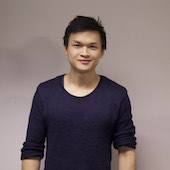
\includegraphics[width=1in,height=1.25in,clip,keepaspectratio]{img/team/Daniel.jpg}}]{Daniel Tran}

Har en bachelor i maskin fra Universitetet i Stavanger, og tar nå en master i materialteknologi på NTNU med fordypning innen materialutvikling og bruk. Siden prosjektet først og fremst handler mye om produktutvikling har Daniel sin ekspertise vært meget nyttig spesielt med tanke på utforming av roboten og finne helhetsforståelse for konseptet.


\end{IEEEbiography}